\documentclass[10pt, handout, xcolor=table]{beamer}

\usepackage[utf8]{inputenc}
\usepackage{amsmath}
\usepackage{amsfonts}
\usepackage{amssymb}
\newcommand*\themecol{\usebeamercolor[fg]{structure}}

\setbeamertemplate{navigation symbols}{}
 \setbeamertemplate{footline}[frame number]



\usepackage{tikz}
\usetikzlibrary{shapes.geometric, arrows}
\tikzstyle{prob} = [rectangle, minimum width=3cm, text width = 4.5cm, minimum height=1cm, text centered, draw=black, fill= blue!20]
\tikzstyle{stat} = [rectangle, minimum width=3cm,  text width = 4.5cm, minimum height=1cm, text centered, draw=black, fill= red!20]
\tikzstyle{arrow} = [thick,->,>=stealth]


\setlength{\parindent}{0pt}
\setlength{\parskip}{6pt}

\title{STAT 111\\
{\small Recitation 1}}

\author{Mo Huang}
\institute{Email: mohuang@wharton.upenn.edu \\
\vspace{0.25cm}
Office Hours: Wednesdays 3:00 - 4:00 pm, JMHH F96\\
\vspace{0.25cm}
Slides (adapted from Gemma Moran): \url{github.com/mohuangx/STAT111-Fall2018} }


\date{September 7, 2018}


\begin{document}

\begin{frame}
\titlepage
\end{frame}



\begin{frame}{Logistics}
  \begin{itemize}
  \item {\themecol Section 201:} 11:00 am - 11:50 am
 \item  {\themecol Section 202:} 12:00 pm - 12:50 pm
 \end{itemize}
 \begin{itemize}
   \setlength{\itemsep}{15pt}
  \item Every Friday, I will:
  \begin{enumerate}
  \item Collect the homework for that week;
  \item Give you your graded homework; and
  \item Give you the homework for the week after (also posted on Canvas).
  \end{enumerate}
  \item If you do not collect your homework, it will be available in the STAT 111 box in the Statistics Department (4th Floor, JMHH).
  \item If you know in advance that you will not be able to attend a recitation, give your homework to Professor Ewens on Thursdays or put it in my mailbox (at entrance to the Statistics Department)
  \item Questions about course materials should be asked during office hours or in an email to Professor Ewens. 
  \end{itemize}
\end{frame}


\begin{frame}{Statistics and Probability}
\begin{itemize}
  \setlength{\itemsep}{20pt}
\item {\themecol Probability theory} is {\em deductive} (or ``top-down logic''). We start with a theory and then consider the implications resulting from that theory. 
\item {\themecol Statistics} is {\em inductive} (or ``bottom-up logic''). We start with finite observations and then attempt to make objective statements about the world from a sample. 
\item Statistical methods use probability theory to draw conclusions from observed data.
\end{itemize}

\end{frame}

\begin{frame}{Statistics and Probability: Example}

\small
\begin{itemize}
  \setlength{\itemsep}{6pt}
\item We currently cure an illness with some medicine (``current medicine'') which cures 80\% of patients.
\item A new medicine is proposed (``new medicine'') which cures 1,643 people out of 2,000.
\end{itemize}
\uncover<2->{{\themecol \bf  Is the new medicine more effective?}}
\uncover<3->{
\begin{center}
{\color{blue!30} Probability theory}
\begin{figure}
\centering
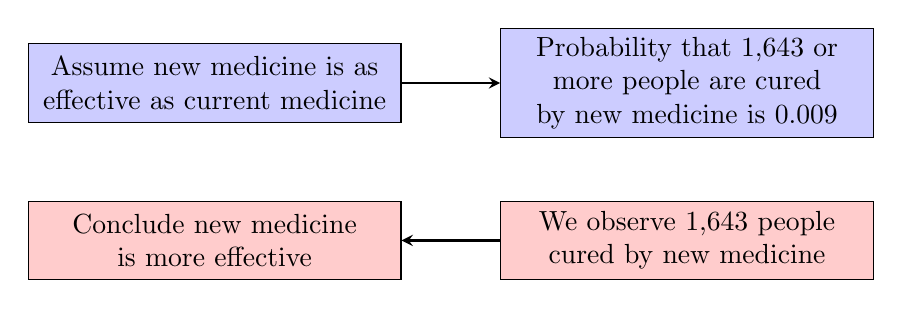
\begin{tikzpicture}[node distance = 2cm]
\node(1)[prob]{Assume new medicine is as effective as current medicine};
\node(2)[prob, right of = 1, xshift = 4cm]{Probability that 1,643 or more people are cured by new medicine is 0.009};
\node(3)[stat, below of = 2]{We observe 1,643 people cured by new medicine};
\node(4)[stat, below of = 1]{Conclude new medicine is more effective};
\draw[arrow](1) -- (2);
\draw[arrow](3) -- (4);
\end{tikzpicture}
\end{figure}
{\color{red!30} Statistics}
\end{center}}

\end{frame}

\begin{frame}{Probability: Axioms}
\pause
\begin{itemize}
  \setlength{\itemsep}{15pt}
\item $0 \leq P(A) \leq 1$, where $A$ is any event.
\item $P(A^C) = 1 - P(A)$ where $A^C$ is the complement of $A$.
\item $P(A \cup B) = P(A) + P(B) - P(A \cap B)$
\end{itemize}
\begin{figure}
\includegraphics[width = 0.9\textwidth]{"images/rec1_1"}
\end{figure}
\end{frame}

\begin{frame}{Probability: Independence}
\pause
\begin{itemize}
  \setlength{\itemsep}{15pt}
\item $A$ and $B$ are independent if and only if $P(A \cap B) = P(A)P(B)$
\item Conditional probability: $P(A|B) = \dfrac{P(A \cap B)}{P(B)}$
\end{itemize}

Suppose $A$ and $B$ are independent. Then
\begin{align*}
P(A|B) = \frac{P(A \cap B)}{P(B)} = \frac{P(A) P(B)}{P(B)} = P(A)
\end{align*}

So we have two definitions of independence:
\begin{enumerate}
\item $P(A \cap B) = P(A)P(B)$
\item $P(A|B) = P(A)$
\end{enumerate}

\textbf{Note:} This year, conditional probability is not on the syllabus but it's still an interesting and useful concept!
\end{frame}

\begin{frame}{Probability: Questions}
\begin{itemize}
  \setlength{\itemsep}{15pt}
\item[Q1:] A smoke alarm consists of two parts, $A$ and $B$. If there is smoke, part $A$ will detect it with probability 0.96 and part $B$ will detect it with probability 0.98. The probability that they both detect it is 0.95. What is the probability that smoke will not be detected?
\item[A1:]<2-> \color{red}
Let A be the event that part A detects smoke and let B be the event that part B detects smoke. What is the event that smoke is not detected?\\
\medskip
\uncover<3->{$A \cup B = \text{Smoke is detected} \to [A \cup B]^C = \text{Smoke is not detected}$}
\uncover<4->{\begin{align*}
P(A \cup B) &= P(A) + P(B) - P(A \cap B) \\
&= 0.96 + 0.98 - 0.95 \\
&= 0.99 \\
P([A \cup B]^C) &= 1 - P(A \cup B) \\
&= 0.01
\end{align*}
}
\end{itemize}
\end{frame}

\begin{frame}{Probability: Questions}
\begin{itemize}
  \setlength{\itemsep}{15pt}
\item[Q2:] A six-sided die is biased such that an odd number is twice as likely to occur as an even number. That is, the probability of an odd number is 2/9 and an even number is 1/9. Let $A$ be the event that an even number occurs. Let $B$ be the event that a number greater than or equal to 4 occurs. Find $P(A)$, $P(B)$, $P(A \cup B)$ and $P(A \cap B)$.
\item<2->[A2:] 
\end{itemize}
\uncover<2->{\color{red}
\begin{columns}
\begin{column}{0.5\textwidth}
\begin{align*}
\uncover<3->{
P(A) &= P(2, 4 \text{ or } 6) \\
&= 1/9 + 1/9 + 1/9 \\
&=3/9} \\
\uncover<5->{
P(A \cap B) &= P(4 \text{ or } 6) \\
&= 1/9 + 1/9 \\
&= 2/9}
\end{align*}
\end{column}
\begin{column}{0.5\textwidth}
\begin{align*}
\uncover<4->{
P(B) &= P(4, 5 \text{ or } 6) \\
&= 1/9 + 2/9 + 1/9\\
&= 4/9}\\
\uncover<6->{
P(A \cup B) &= P(A) + P(B) - P(A \cap B) \\
&= 3/9 + 4/9 - 2/9 \\
&= 5/9}
\end{align*}
\end{column}
\end{columns}}
\end{frame}

\begin{frame}{Probability: Questions}
\bigskip
\begin{itemize}
\setlength{\itemsep}{15pt}
\item[A2:] {\color{red} $P(A) = 3/9, \quad P(B) = 4/9, \quad P(A \cap B) = 2/9, \quad P(A \cup B) = 5/9$}
\item[Q3:] Following Q2, find $P(A|B)$.
\item[A3:]<2->{ \color{red}
\begin{align*}
P(A|B) &= \frac{P(A \cap B)}{P(B)} \\
&= \frac{2/9}{4/9}\\
&= 1/2
\end{align*}}
\item[Q4:]<3-> Are $A$ and $B$ independent?
\item[A4:]<4-> {\color{red} No, because $P(A|B) \neq P(A)$. (Recall $P(A) = 1/3$).}
\end{itemize}
\end{frame}

\begin{frame}{Probability: Questions}

\begin{itemize}
  \setlength{\itemsep}{15pt}
\item[Q5:] An unfair coin ($P(H) = 0.4$) was flipped twice. Given that on at least one flip a head occurred, what is the probability that a head occurred on both flips?
\item[A5:]<2-> \color{red} 
We want to find $P(HH | \text{at least one } H)$.
\uncover<3->{
\begin{align*}
P(\text{at least one }H) &= P(HH) + P(HT) + P(TH)\\
&= (0.4)^2 + (0.4)(0.6) + (0.6)(0.4) \\
&= 0.64.\\ 
\uncover<4->{
P(HH|\text{at least one }H) &= \frac{P(HH \cap \text{at least one }H)}{P(\text{at least one }H)} \\
&= \frac{P(HH)}{P(\text{at least one }H)} \\
&= \frac{(0.4)^2}{0.64} \\
&= 0.25}
\end{align*}
}
\end{itemize}
\end{frame}

\begin{frame}{Parameters ($\theta$), Random Variables ($X$), and Data ($x$)}
\begin{itemize}\itemsep1ex
\item<1-> A {\themecol parameter} represents some underlying numerical constant of a phenomenon. Represented by Greek letters.
\item<3-> A {\themecol random variable} is a numerical outcome of interest in a future experiment. Can be modeled by a probability {\themecol distribution} which depends on the parameter. Represented by capital letters.
\item<5-> {\themecol Data} is the realization or observed value of a random variable after performing the experiment. Represented by lower-case letters.
\end{itemize}

\bigskip
\only<2->{Fair coin-flipping example:}
\begin{itemize}\itemsep1ex
\item<2-> A {\themecol parameter} $\theta$ is the underlying probability of obtaining a head. $\theta = 0.5$.
\item<4-> A {\themecol random variable} $X$ is the number of heads obtained in 10 tosses. Can be modeled by a binomial distribution dependent on $\theta$.
\item<6-> {\themecol Data} $x=6$ is observing 6 heads in 10 tosses, a realization of $X$.
\end{itemize}
\end{frame}

\begin{frame}{Random Variables}
\begin{itemize}\itemsep1ex
\item<1-> Two types of random variables: {\themecol discrete} and continuous.
\item<1-> A {\themecol discrete random variable} is a random variable that can only take on a countable set of numbers.
\item<1-> The {\themecol probability distribution} of a discrete random variable is the range of values it can take \emph{and} the probabilities of these values.
\item<2-> For example:
\begin{itemize}
\vspace{0.25cm} \color{blue!70}
\item Let $X$ be the number of heads I toss if I toss a fair coin 3 times.
\end{itemize}
\end{itemize}
\uncover<3->{
\begin{table}
\begin{tabular}{|c|c|c|c|c|}
\hline
\rowcolor{blue!10} $x$ & 0 & 1& 2&3  \\ \hline
$P(X = x)$ & 0.125 & 0.375 & 0.375 &0.125 \\
\hline
\end{tabular}
\caption{Probability distribution of $X$.} 
\end{table}}
\end{frame}

\begin{frame}{Random Variables: Mean}
\begin{itemize}
\setlength{\itemsep}{15pt}
\item<1-> The {\themecol mean of a random variable} (expected value) is the long-run average of realizations of the random variable over repeated experiments.
\item<2-> This mean of random variable $X$ is different from the sample mean, which is the average of a \emph{finite} number of observations ($x$).
\item<3-> Let $X$ be a discrete random variable that can take values $\{v_1,v_2,\dots, v_k\}$. Then the mean of $X$ is given by:
\begin{align*} 
\mu &= \sum_{i = 1}^k v_i P(X = v_i)\\
&= v_1P(X = v_1) + v_2P(X = v_2) + \cdots + v_kP(X = v_k).
\end{align*}
\begin{itemize}
\item[Note:] We use $\mu$ to denote the mean of a random variable.
\item[Note:] Can think of it as a weighted average, weighted by probability.
\end{itemize}
\end{itemize}
\end{frame}




\begin{frame}{The Binomial Distribution}
\begin{itemize}
\setlength{\itemsep}{15pt}
\item The {\themecol binomial distribution} arises if:
\begin{enumerate}
\vspace{0.25cm}
\setlength{\itemsep}{6pt}
\item<2-> We plan to conduct a fixed number of experiments. We denote the number of experiments as $n$.
\item<3-6,8-> In each experiment, there are two outcomes: ``success'' or ``failure".
\item<4-6, 9-> The experiments are independent.
\item<5-6, 10-> The probability of a success is the same for each experiment.
\end{enumerate}
\item<6-> For example: 
\begin{enumerate} \color{blue!70}
\vspace{0.25cm}
\setlength{\itemsep}{6pt}
\item<7-> I plan to toss a coin $n$ times.
\item<8-> I can toss either a head or a tail.
\item<9-> Each coin toss is independent of the next - it doesn't matter whether I get a head or a tail on the previous toss.
\item<10-> The probability of getting a head is the same for each toss.
\end{enumerate}
\end{itemize}
\end{frame}

\begin{frame}{The Binomial Distribution}
\begin{itemize}
\setlength{\itemsep}{15pt}
\item Let $X$ be a binomial random variable where $\theta = P(\text{success})$ and there are $n$ experiments. Then the probability distribution of $X$ is given by:
$$ P(X = x) = {n \choose x} \theta^x (1-\theta)^{n-x}, \quad \text{for } x = 0, 1, 2, \dots, n.$$
\begin{itemize}
\setlength{\itemsep}{6pt}
\item<2-> $\theta$ is called a {\themecol parameter}: a constant whose value may be known or unknown.
\item<3-> ${n \choose x}$ is said as ``$n$ choose $x$'': it is the number of ways $x$ successes can occur in $n$ experiments.
\end{itemize}
\item<4->[Note:] $X \sim \mathcal{B}(n, \theta)$ means ``$X$ is a binomial random variable with $n$ experiments and probability of success $\theta$.''
\end{itemize}
\end{frame}


\begin{frame}{The Binomial Distribution: Mean}
\begin{itemize}
\setlength{\itemsep}{20pt}
\item For the binomial distribution, we have a simpler formula for the mean: if $X\sim \mathcal{B}(n, \theta)$, then the mean of $X$ is
\begin{align*}
\mu = n\theta.
\end{align*}
\item<2-> For example: 
\begin{itemize}
\item \color{blue!70} On the previous slide, we calculated the mean of a binomial random variable with $n = 3$ and $\theta = 0.5$ to be 1.5. This is exactly $n\theta$. 
\end{itemize}
\vspace{0.5cm}
\begin{itemize}
\item<3->[Note:] This formula is \emph{only} for the binomial distribution.
\end{itemize}
\end{itemize}
\end{frame}


\end{document}


